\documentclass[11pt,letterpaper]{article}
\usepackage[lmargin=1in,rmargin=1in,tmargin=1in,bmargin=1in]{geometry}
\usepackage{../style/quiz}
\setbool{hideans}{true} % Student: True; Instructor: False

% -------------------
% Content
% -------------------
\begin{document}
\quiz{1}

\problem Consider the plot of the relation $f(x)$ shown below. 
	\[
	\fbox{
	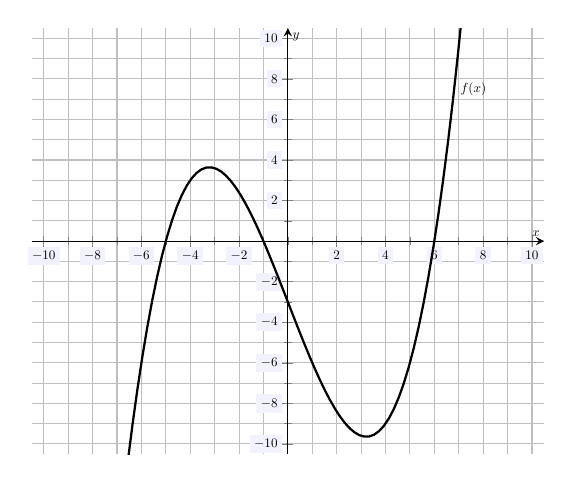
\begin{tikzpicture}[scale=0.95,every node/.style={scale=0.5}]
	\begin{axis}[
	grid=both,
	axis lines=middle,
	ticklabel style={fill=blue!5!white},
	xmin= -10.5, xmax=10.5,
	ymin= -10.5, ymax=10.5,
	xtick={-10,-8,...,10},
	ytick={-10,-8,...,10},
	minor tick = {-10,-9,...,10},
	xlabel=\(x\),ylabel=\(y\),
	]
	\node at (7.6,7.5) {$f(x)$};
	\addplot[line width= 0.03cm,samples=100,domain= -10:10] ({x},{1/10*(x+1)*(x + 5)*(x-6)});

	\end{axis}
	\end{tikzpicture}
	}
	\]

\begin{enumerate}[(a)]
\item Is the relation $f(x)$ a function? Explain.
	
	\ans{Yes, $f(x)$ is a function because it passes the Vertical Line Test---every vertical line intersects the function at most once.}

\item Find the $x$-intercepts. 

	\ans{The $x$-intercepts are where $f(x)$ intersects the $x$-axis, which is at $-5, -1, 6$.}

\item Find the $y$-intercepts. 

	\ans{The $y$-intercepts are where $f(x)$ intersects the $y$-axis, which is at $-3$.}
\end{enumerate} \pspace


\problem There are two relations, $f$ and $g$, shown below. Only one of these relations is \textit{not} a function. Identify which is \textit{not} a function. Being as specific as possible, explain why that relation is not a function.
	\[
	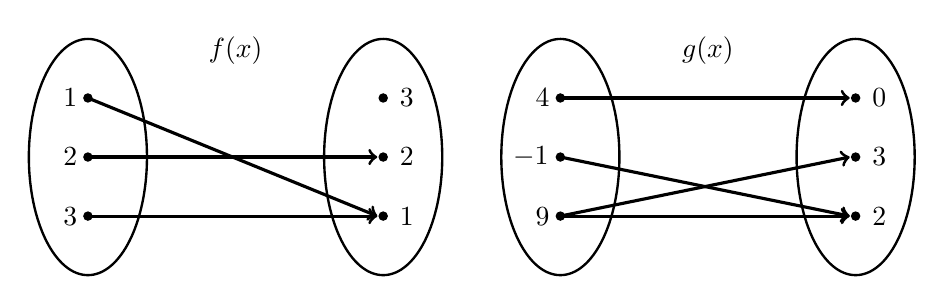
\begin{tikzpicture}[scale=0.75]
	\node at (2.5,1.8) {$f(x)$};
	% Ellipses
	\draw[line width=0.03cm] (0,0) circle (1 and 2);
	\draw[line width=0.03cm] (5,0) circle (1 and 2);
	
	% Nodes
	\draw[fill=black] (0,1) circle (0.07);
	\draw[fill=black] (0,0) circle (0.07);
	\draw[fill=black] (0,-1) circle (0.07);
	
	\draw[fill=black] (5,1) circle (0.07);
	\draw[fill=black] (5,0) circle (0.07);
	\draw[fill=black] (5,-1) circle (0.07);
	
	% Arrow
	\draw[line width=0.04cm,->] (0,1) -- (4.9,-1);
	\draw[line width=0.04cm,->] (0,0) -- (4.9,0);
	\draw[line width=0.04cm,->] (0,-1) -- (4.9,-1);
	
	% Labels
	\node at (-0.3,1) {$1$};
	\node at (-0.3,0) {$2$};
	\node at (-0.3,-1) {$3$};
	
	\node at (5.4,1) {$3$};
	\node at (5.4,0) {$2$};
	\node at (5.4,-1) {$1$};
	
	\tikzset{shift={(8,0)}}
	%
	\node at (2.5,1.8) {$g(x)$};
	% Ellipses
	\draw[line width=0.03cm] (0,0) circle (1 and 2);
	\draw[line width=0.03cm] (5,0) circle (1 and 2);
	
	% Nodes
	\draw[fill=black] (0,1) circle (0.07);
	\draw[fill=black] (0,0) circle (0.07);
	\draw[fill=black] (0,-1) circle (0.07);
	
	\draw[fill=black] (5,1) circle (0.07);
	\draw[fill=black] (5,0) circle (0.07);
	\draw[fill=black] (5,-1) circle (0.07);
	
	% Arrow
	\draw[line width=0.04cm,->] (0,1) -- (4.9,1);
	\draw[line width=0.04cm,->] (0,0) -- (4.9,-1);
	\draw[line width=0.04cm,->] (0,-1) -- (4.9,0);
	\draw[line width=0.04cm,->] (0,-1) -- (4.9,-1);
	
	% Labels
	\node at (-0.3,1) {$4$};
	\node at (-0.5,0) {$-1$};
	\node at (-0.3,-1) {$9$};
	
	\node at (5.4,1) {$0$};
	\node at (5.4,0) {$3$};
	\node at (5.4,-1) {$2$};
	\end{tikzpicture}
	\] \pspace

\ans{The relation $g(x)$ is not a function. This is because not every input goes to only one output. For example, $g(9)$ is not well defined because it has two possible outputs: 3 and 2.}

\end{document}